\chapter{光的粒子性}
光的电磁说使光的波动理论发展到相当完美的地步,取
得了巨大成就.但是,这个学说并不能完美地解释所有的光
现象,还在赫兹用实验证实光的电磁说的时候,就已经发现了
后来叫做光电效应的现象,这个现象使光的电磁说遇到了无
法克服的困难.二十世纪初,人们在新的事实的基础上建立了
关于光的新的学说——光子说,对光的本性的认识又前进了
一步.


\section{光电效应}
1887年,赫兹在进行电磁波的实验时发现了一个奇妙的
现象:当紫外线照射到圆环接收器间隙的电极上时,火花放电
变得容易了,后来其他科学家又发现,用紫外线照射与验电
器相连的带负电的锌板时,验电器的金箔便立即闭合.用紫
外线照射与验电器相连的不带电的锌板时,验电器上带正电.
通过这些现象人们认识到,用紫外线照射金属时,电子会从金
属表面飞出来.在紫外线照射下,赫兹实验中的电极变得容
易放电,带负电的锌板失去电荷,不带电的锌板带上了正电,
都是由于电子从金属表面飞出来了的缘故.
\begin{figure}[htp]\centering
    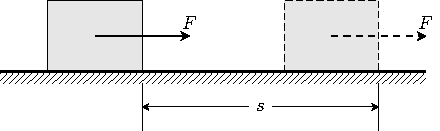
\includegraphics[scale=.6]{fig/7-1.png}
    \caption{紫外线照射锌板使验电器带正电}
    \end{figure}

在光的照射下物体中发射电子的现象,叫做\textbf{光电效应}.光
电效应中发射出来的电子叫做\textbf{光电子}.实验表明,不仅紫外
线能产生光电效应,对于碱金属,例如锂、钠、钾、铯等,用可见
光照射也能产生光电效应.
\begin{figure}[htp]\centering
    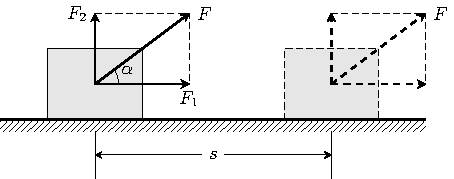
\includegraphics[scale=1.2]{fig/7-2.pdf}
    \caption{研究光电效应的装置简图}
    \end{figure}

图7.2是研究光电效应规律的实验装置简图,其中$S$是
抽成真空的容器,$C$是石英窗口,紫外光和可见光都可以通过
它射到容器里的金属板$K$上.在$K$的对面有另一金属板$A$,$K$
和$A$组成一对电极.象图中那样把$K$跟电池组的负极相连,
$A$正极相连,电路接好后,电流表指示没有电流,因为极板
$K$和$A$之间是断开的,用一定强度的光照射极板$K$,它发射
出的光电子运动到极板$A$时,电流表的指针就发生偏转,指出
电路中产生了电流,这电流是由光电子产生的,叫做光电流.

逐渐增加极板$K$和$A$间的正向电压(使$A$板电势比$K$板
高),电路里的光电流也逐渐增大.当正向电压增到几伏时,
光电流就达到最大值——饱和值.再增加电压,光电流也不
再增大了,这表明$K$板发射的光电子已全部被$A$板吸去.这
时增加入射光的强度,光电流值就继续上升.入射光的强度
增加一倍,光电流的饱和值也增加一倍,这表明,\textit{在单位时间
里从极板$K$发射出的光电子数跟入射光的强度成正比}.

逐渐减小极板$K$和$A$间的正向电压,当这电压减小为零
时,电路里仍有相当强的光电流.可见光电子从极板$K$飞出
时具有某种初动能,没有正向电场的作用,也有相当数量的光
电子到达极板$A$.要完全阻止光电流,必须在$KA$间加一定
的反向电压(使$A$板电势低于$K$板电势),使那些具有最大初
动能的光电子不足以克服反向电场的阻力而到达极板$A$,就
没有光电流了.这时,光电子的最大初动能
$\dfrac{1}{2}mv^2_m$
与反向电压$U$
之间有下面的关系:
\[\dfrac{1}{2}mv^2_m=eU \]
式中的$e$表示电子的电量.
因此,从实验中测出使光电流减小到零时的反向电压$U$的值,
就可以求出光电子的最大初动能.实验表明,\textit{光电子的最大初
动能与入射光的强度无关,只随着入射光频率的增大而增大}.

换用不同材料的极板$K$重做实验,结果表明,光电子的最
大初动能还跟极板$K$的材料有关.\textit{对于任何一种金属,入射光
的频率必须大于某一极限频率才能产生光电效应;低于这个
极限频率的光,无论强度如何,照射时间多长,也不能产生光
电效应}.
下表是几种金属的极限频率$\nu_0$和波长$\lambda_0$.
\begin{center}
    \begin{tabular}{cccccc}
        \hline
        金属& $\lambda_0$(微米)& $\nu_0$(赫)\\
        \hline
        铯&0.66&$4.545\x 10^{14}$ \\
        钠&0.50&$6.000\x 10^{14}$\\
        锌&0.37&$8.065\x 10^{14}$\\
        银&0.26&$1.153\x 10^{15}$\\
        铂& 0.20&$1.529\x 10^{15}$\\
        \hline
    \end{tabular}
\end{center}



\section{爱因斯坦对光电效应的解释}
\subsection{光子}
光电效应的规律无法用经典的波动理论来解释.按照波
动理论,光的能量是由光的强度决定的,而光的强度又是由光
波的振幅决定的,跟频率无关.因此,不论光的频率如何,只
要光的强度足够大或照射时间足够长,都应该有足够的能量
产生光电效应,然而这跟实验结果是直接矛盾的.极限频率
的存在,即频率低于某一数值的光不论强度如何都不能产生
光电效应,这是波动理论不能解释的.

对光电效应的解释是1905年爱因斯坦(1879—1955)在
普朗克(1858—1947)的量子论的基础上作出的.1900年德国
物理学家普朗克在研究电磁辐射的规律时发现,只有假设电
磁辐射的能量是不连续的,而是一份一份地进行的,每一份的
能量是$h\nu$,其中$\nu$是辐射的频率,是一个普适恒量,理论计
算的结果才能跟实验事实很好地符合.这个$h$后来就叫做\textbf{普
朗克恒量},实验测出$h=6.63\x10^{-34}{\rm J}\cdot {\rm s}$,在普朗克的量
子说的启发下,爱因斯坦天才地预见到,为了解释光电效应必
须假设光也是不连续的,而是一份一份的,每一份光叫做一个
\textbf{光子},光子的能量跟它的频率成正比,即$E=h\nu$,其中的$h$是
普朗克恒量.这就是爱因斯坦在1905年提出的光子说.爱
因斯坦是在实验事实还不很充分的情况下做出这一假设的,
但是从这个假设得出的一切结论都跟后来的实验结果相符.

光子说很好地解释了光电效应,当光子照射到金属上
时,它的能量可以被属中的某个电子全部吸收,电子吸收
光子的能量后,动能就增加了,如果电子的动能足够大,能够克
服内部原子对它的引力,就可以离开金属表面逃逸出来,成为
光电子,这就是光电效应,电子吸收光子的能量后可能向各
个方向运动,有的向金属内部运动,并不出来,向金属表面运
动的电子,经过的路程不同,途中损失的能量也不同,因此从
表面出来时的初动能也不同,只有直接从金属表面出来的光
电子才具有最大初动能,这些光电子克服金属原子的引力
所做的功叫做\textbf{逸出功},根据能量守恒定律,光电子的最大初
动能跟入射光子的能量$h\nu$和逸出功$W$之间有下面的关系:
\[\frac{1}{2}mv^2_m=h\nu-W \]
这个方程叫做爱因斯坦\textbf{光电效应方程}.

对于一定的金属来说,逸出功$W$的值是一定的,所以,入
射光子的频率$\nu$越大,光电子的最大初动能也越大,如果入
射光子的频率比较低,它的能量小于金属的逸出功,就不能产
生光电效应了,这就是存在极限频率的原因.极限频率$\nu_0$可
由下式求出:
\[h\nu_0=W\quad \Rightarrow\quad \nu_0=\frac{W}{h} \]

不同金属的逸出功不同,所以它们的极限频率也不同,如
果入射光比较强,即单位时间内入射光子的数目多,产生的光
电子也多,所以光电流的饱和值也大.

\subsection*{练习一}

\begin{enumerate}
    \item 使锌板产生光电效应的光子的最长波长是0.37微
米,这种光子的能量是多少电子伏?锌的逸出功是多少?
\item 可见光的光子,能量范围是多大(用电子伏表示)?为
什么用可见光不能使锌板产生光电效应?
\item 铯的逸出功是$3.0\x10^{-19}$焦,用波长是0.59微米的
黄光照射铯,电子从绝表面飞出的最大初动能是多大?
\item 钨的逸出功是4.52电子伏,使钨产生光电效应的最
长波长是多少?这种波长是可见光吗?
\end{enumerate}

\section{光电效应的应用}

利用光电效应可以把光信号转变为电信号,动作迅速灵
敏,因此利用光电效应制作的光电器件在工农业生产,科学技
术和文化生活领域内得到了广泛的应用,光电管就是应用最
普遍的一种光电器件.

光电管的类型很多.图7.3甲是其中的一种,玻璃泡里
的空气已经抽出,有的管里充有少量的惰性气体(如氩、氖、氦
等),管的内半壁涂有逸出功小的碱金属作为阴极$K$,管内
另有一阳极$A$.使用时照图7.3乙那样把它连在电路里,当
光照射到光电管的阴极$K$时,阴极发射电子,电路里就产生电
流,光电管不能受强光照射,否则容易老化失效.光电管产生
的电流很弱,应用时可以用放大器把它放大.
\begin{figure}[htp]\centering
    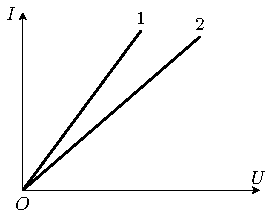
\includegraphics[scale=.7]{fig/7-3.png}
    \caption{光电管}
    \end{figure}

下面举例说明光电管的应用.

\subsection{光控继电器}

工业生产中的大部分光电控制设备都用光
控继电器.图7.4是光控继电器的示意图,它由电源、光电
管、放大器、电磁继电器几部分组成.当光照射光电管时,光
放大器电管电路中便产生电流,经放大器放大后,使电磁铁$M$磁化,
把衔铁$N$吸住;没有光照射光电管时,电路中没有电流,衔铁
$N$在弹簧的作用下就自动离开$M$.如果把衔铁$N$跟控制机构
相连,就可以达到自动控制的目的.
\begin{figure}[htp]\centering
    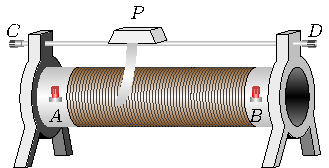
\includegraphics[scale=1.2]{fig/7-4.PDF}
    \caption{光控继电器示意图}
    \end{figure}


光控继电器在工业上可以用于产品的自动计数、安全生
产等方面,用于自动计数时,可以把产品放在传送带上,光源
和光电管分别放在传送带的两侧,每当传送带上输送过去一
个产品时,光线被挡住一次,光控继电器就放开衔铁一次,由
衔铁控制的计数器的数字就加一.工人在冲床、钻床、锻压机
械上劳动时,如有不慎,容易出事故.为保证安全,可以在这些
机床上安装光控继电器,当工人不慎将手伸人危险部位时,
由于遮住了光线,光控继电器就立即动作,使机床停下来,避
免事故的发生.


\subsection{有声电影}

最早的电影是没有声音的,后来虽然有了声
音,但那是靠留声机来配合影片播放的,声和影配合不好时,
效果当然不好,我们现在能够看到声和影完全配合一致的有
声电影,还是多亏了光电管.

影片摄制完后,要进行录音,录音时通过专门的设备使声
音的变化转变成光的变化,从而把声音的“像”摄制在影片的
边缘上,形成宽窄变化的暗条纹,这就是影片边上的\textbf{音道}.

放映电影时,利用光电管把“声音的照片”还原成声音.方
法是:在电影放映机中用强度不变的极窄的光束照射音道,
由于影片上各处的音道宽窄不同,所以在影片移动的过程中,
通过音道的光的强度也就不断变化;变化的光射向光电管时,
在电路中产生变化的电流,把电流放大后,通过喇叭就可以把
声音放出来.

\section{光的波粒二象性}
光的干涉、衍射和偏振等现象无可争辩地表明光具有波
动性,而光电效应又无可争辩地表明光是具有能量$E=h\nu$的
光子流,也就是说光具有粒子性.这样,已经退出历史舞台的
光的微粒说,在二十世纪初又以新的形式被重新提了出来.当
然人们现在对光的粒子性的认识比起十七世纪牛顿提出微粒
说时已经大不相同.人类对光的本性的认识经过曲折的发展
过程已经越来越深入了.现在,人们认识到,光既具有波动
性,又具有粒子性,也就是说,\textit{光具有波粒二象性}.

十七世纪的微粒说和波动说是互相对立的两种学说,都
企图用一种观点去说明光的本性,这是受了传统观念的影响.
传统观念是我们在观察周围世界的宏观现象中形成的,波动
性和粒子性在宏观现象中是互相对立的、矛盾的,没有任何宏
观物体既有波动性、又有粒子性.对于宏观物体来说,波粒二
象性是不可想像的.

但是,对于光子这样的微观粒子,却只有从波粒二象性出
发,才能说明它的各种行为.实际上,光子说并没有否定光的
电磁说,光子的能量$E=h\nu$,其中的频率$\nu$表示的仍是波的特
征.此外,从光子说和电磁说还往往得到一致的结论.例如,
光子说和电磁说都可以推导出光具有动量,并且为实验所证
实,光子说的结论是光子的动量$p=h\nu/c$,
电磁说的结论是辐射
能$E$具有的动量是$p=E/c$.由于光子的能量$E=h\nu$,所以从
这两个学说得到的结论是一致的,由于$c=\lambda\nu$,光子的动量
也可以写成
$$p=\frac{h}{\lambda}$$
式中的波长$\lambda$表示的也是波的特征.可
见,对于宏观物体来说不可想像的波粒二象性,在微观世界却
是不可避免地必须予以承认的现实,接受光的波粒二象性,
就要求我们既不可把光当成宏观观念中的波,也不可把光当
成宏观观念中的粒子.

那么,在微观世界中,波和粒子又是怎样统一起来的呢?
物理学家做的下述实验可以帮助我们理解这个问题.在光的
双缝干涉实验中,在像屏处放上照相底片,并设法减弱光流的
强度,由于每个光子的能量$h\nu$可以从频率$\nu$算出,因此进一
步从光流的能量可以算出所含光子的数目.这样就可以使光
流减弱到使光子只能一个一个地通过狭缝,实验结果表明,
如果曝光时间不太长,底片上只出现一些无规则分布的点子,
那些点子是光子打在底片上形成的,表现出光的粒子性,这
些点子的分布是无规则的,可见光子的运动跟我们在研究宏
观现象时假设的质点的运动不同,没有一定的轨道,如果嘲光
时间足够长,底片上就出现了规则的干涉条纹,就象用强光
经短时间曝光后产生的一样,可见,光的波动性是大量光子
表现出来的现象.在干涉条纹中,那些光波强度大的地方,也
就是光子到达机会多的地方,或者说,是光子到达的几率大的
地方;光波强度小的地方,是光子到达的几率小的地方,所以
从这种意义上,可以把光的波动性看做是表明大量光子运动
规律的一种\textbf{几率波}.

一般说来,大量光子产生的效果往往显示出波动性,个别
光子产生的效果往往显示出粒子性,让我们稍稍详细地说明
一下.

无线电波的频率较低,波长较长,这种电磁波的“光子”的
能量很低,以频率为1兆赫的无线电波来说,它的“光子”的能
量只有$4\x10^{-9}$电子伏,能量这样低,只有非常大量的“光
子”才能使接收装置发生反应.较好的接收机大约要每秒收
到$10^{10}$个这样的“光子”才起作用,所以,这部分电磁波的波
动性很容易观察到,要观察这部分电磁波的粒子性,觉察个别
“光子”的作用,却是非常不容易的.

可见光的频率范围大致是$4\x10^{14}$—$8\x10^{14}$赫,这种光
子的能量大约是几个电子伏.人造的仪器设备既可以比较容
易地探测到大量的这种光子的作用,也可以比较容易地探测
到少数这种光子的作用,因此这种电磁波的波、动性和粒子性
都能够比较容易地观察到.

随着电磁波频率的增大,波长越来越短,波动性就越来越
不显著,而粒子性却越来越明显了.伦琴射线的光子的能量
大约是几千电子伏,$\gamma$射线的光子的能量在几兆电子伏以上.
个别$\gamma$射线的光子很容易探测出来,而要看到它们的干涉、衍
射现象却很困难了.伦琴射线只有用晶体作衍射光栅才能看
到衍射图样,因为晶体内粒子间的距离恰好是$10^{-10}$
米左右.至于$\gamma$射线,连用晶体作衍射光栅也不行,因为晶体里粒子间
的距离,比它的波长大得不可比拟.

总之,要理解各种频率的电磁波,我们必须综合运用波动
的观点和粒子的观点,而且要注意到,这里的波动并不等同
于宏观世界里的机械波,这里的粒子也不等同于宏观世界里
的质点.

\section{物质波}
在光具有波粒二象性的启发下,法国物理学家德布罗意
(1892—1987)在1924年提出一个假说,指出波粒二象性不只是光
子才有,一切微观粒子,包括电子和质子、中子,都有波粒二象
性.他把光子的动量与波长的关系式$p=h/\lambda$
推广到一切微观
粒子上,指出:具有质量$m$和速度$v$的运动粒子也具有波动
性,这种波的波长等于普朗克恒量$h$跟粒子动量$mv$的比,即
\[\lambda=\frac{h}{mv} \]
这个关系式后来就叫做德布罗意公式.

从德布罗意公式很容易算出运动粒子的波长.例如,电
子的电荷是$1.6\x10^{-19}$
库,质量是$0.91\x10^{-30}$千克,经过200
伏电势差加速的电子获得的能量
\[E=Ue=200\x1.6\x10^{-19}=3.2\x10^{-17}{\rm J}\]
这个能量就是电子的动能,即
\[\dfrac{1}{2}mv^2=3.2\x10^{-17}{\rm J} \]
因此
\[v=\sqrt{\frac{2\x 3.2\x10^{-17}}{0.91\x 10^{-30}}}=8.4\x10^6\ms \]
于是,按照德布罗意公式这运动电子的波长是
\[\begin{split}
    \lambda=\dfrac{h}{mv}&=\frac{6.63\x 10^{-34}}{0.91\x10^{-30}\x8.4\x 10^6}{\rm m} \\
&=8.7\x10^{-11}{\rm m}=0.87\text{\AA}
\end{split}\]
我们看到,这个波长与伦琴射线的波长相仿.前面讲过,这样
短的波长,只有用晶体做衍射光栅才能观察到衍射现象.后
来人们的确用这种办法观察到了电子的衍射,从而证明了德
布罗意假说的正确性.
\begin{figure}[htp]\centering
    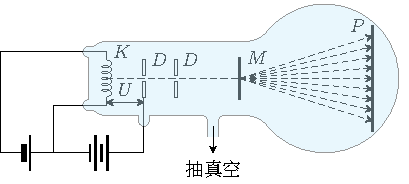
\includegraphics[scale=.7]{fig/7-5.png}
    \caption{电子衍射实验示意图}
    \end{figure}

图7.5是一种电子衍射实验的示意图,从灯丝$K$发射出
的电子经过电势差为$U$的加速电场,然后通过一组栏板$D$的
小孔,成为很细的电子束射到铝箔$M$上,在铝箔的后面放一
张照相底片$P$,于是就得到图7.6所示的照片,在中央斑点
的周围出现了环形的明暗相间的花纹.这个衍射图样跟伦琴
射线穿过同一铝箔后产生的衍射图样(图7.7)非常相似,这
是电子具有波动性的证明.根据铝箔原子间的距离、加速电
势差和衍射条纹的几何图形,还可以算出电子衍射时的波长,
实测结果跟德布罗意公式相符.
\begin{figure}[htp]
    \centering
    \begin{minipage}[t]{0.48\textwidth}
    \centering
    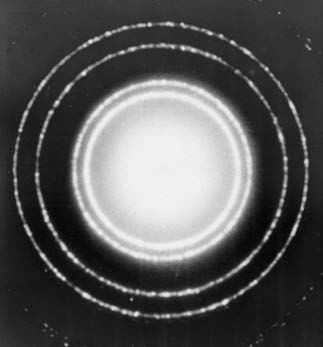
\includegraphics[scale=.8]{fig/7-6.jpg}
    \caption{电子衍射图样}
    \end{minipage}
    \begin{minipage}[t]{0.48\textwidth}
    \centering
    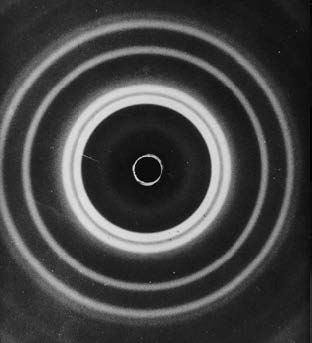
\includegraphics[scale=.8]{fig/7-7.jpg}
    \caption{伦琴射线衍射图样}
    \end{minipage}
    \end{figure}


后来人们又用原子射线和分子射线做类似的实验,同样
得到了衍射图样,质子和中子的衍射实验也做成功了,这就
证明了一切运动的微观粒子都具有波粒二象性,其波长与动
量的关系都符合德布罗意公式,于是人们就把这种波叫做德
布罗意波或\textbf{物质波}.

那么,物质波是一种什么波呢?我们知道,机械波是周期
性的振动在媒质内的传播,电磁波是周期变化的电磁场的传
播,物质波既不是机械波,也不是电磁波,在德布罗意提出
物质波以后,人们曾经对它提出过各种各样的解释,到1926
年,德国物理学家玻恩(1882—1970)提出了符合实验事实的
后来为大家公认的统计解释:物质波在某一地方的强度跟在
该处找到它所代表的粒子的几率成正比,按玻恩的解释,\textit{物
质波乃是一种几率波}.

牛顿力学完全不能解释电子等微观粒子的衍射现象,用
物质波的统计解释却很容易说明这种现象,在图7.5的实验
里,电子流通过金属箔片以后,物质波发生衍射,有的地方由
于波的叠加而使物质波的强度增大,电子到达这里的几率就
大,因而到达这里的电子数较多,有的地方由于波的叠加而
使物质波的强度减小甚至等于零,电子到达这里的几率就较
小甚至等于零,因面到达这里的电子数很少甚至没有.

发现了电子、质子等微观粒子的波动性以后,我们对微观
世界的认识统一起来了,不但原来认为是电磁波的光具有粒
子性,而且原来认为是粒子的电子、质子等也具有波动性.当
然,应该指出,虽然所有的微观粒子都具有波粒二象性,但光
子跟电子、质子等粒子还是有很基本的区别的,光子没有静
质量,电子、质子等都有静质量.光子的运动速度永远是$c$,
电子、质子等却可以有低于光速$c$的各种不同的运动速度.

\section*{复习题}
\begin{enumerate}
\item 什么是光电效应?光电效应有哪些重要的规律?这些
规律中哪些是波动说无法解释的?
\item 什么是光子说?光子说是怎样解释光电效应的?写出
光电效应方程
\item 说明光电管的结构和原理,并举例说明它的应用.
\item 为什么说光具有波粒二象性?应该怎样理解光的波
粒二象性?
\item 德布罗意提出的物质波的含义是什么?什么实验证
明了德布罗意物质波假设的正确性?
\end{enumerate}

\section*{习题}
\begin{enumerate}
    \item 功率为1瓦的手电筒灯泡大约有5\%的电能转化为
可见光,试估算它1秒钟能释放出多少个可见光的光子.
\item 使铜产生光电效应的最低频率是$1.1\x10^{15}$
赫,用频率为$1.5\x10^{15}$赫的紫外线照射铜时,它发射出的光电子的
最大速度是多大?
\item 一个质量为$4\x10^{-4}$克的尘埃颗粒,以$1{\rm cm}/{\rm s}$
的速度在空气中下落,计算它的德布罗意波长.
\item 计算速度为$10^3\ms$的中子的德布罗意波长.这
个波长跟$\gamma$射线的波长相比如何?中子的质量是$1.67\x10^{-27}$
kg.
\end{enumerate}






















